% Options for packages loaded elsewhere
\PassOptionsToPackage{unicode}{hyperref}
\PassOptionsToPackage{hyphens}{url}
\PassOptionsToPackage{dvipsnames,svgnames,x11names}{xcolor}
%
\documentclass[
  a4paper,
]{article}

\usepackage{amsmath,amssymb}
\usepackage{iftex}
\ifPDFTeX
  \usepackage[T1]{fontenc}
  \usepackage[utf8]{inputenc}
  \usepackage{textcomp} % provide euro and other symbols
\else % if luatex or xetex
  \usepackage{unicode-math}
  \defaultfontfeatures{Scale=MatchLowercase}
  \defaultfontfeatures[\rmfamily]{Ligatures=TeX,Scale=1}
\fi
\usepackage{lmodern}
\ifPDFTeX\else  
    % xetex/luatex font selection
\fi
% Use upquote if available, for straight quotes in verbatim environments
\IfFileExists{upquote.sty}{\usepackage{upquote}}{}
\IfFileExists{microtype.sty}{% use microtype if available
  \usepackage[]{microtype}
  \UseMicrotypeSet[protrusion]{basicmath} % disable protrusion for tt fonts
}{}
\makeatletter
\@ifundefined{KOMAClassName}{% if non-KOMA class
  \IfFileExists{parskip.sty}{%
    \usepackage{parskip}
  }{% else
    \setlength{\parindent}{0pt}
    \setlength{\parskip}{6pt plus 2pt minus 1pt}}
}{% if KOMA class
  \KOMAoptions{parskip=half}}
\makeatother
\usepackage{xcolor}
\usepackage[paperwidth=8.27in,paperheight=11.69in,left=1.25in,textwidth=
5.25in,top=1.00in,textheight=8.25in]{geometry}
\setlength{\emergencystretch}{3em} % prevent overfull lines
\setcounter{secnumdepth}{5}
% Make \paragraph and \subparagraph free-standing
\makeatletter
\ifx\paragraph\undefined\else
  \let\oldparagraph\paragraph
  \renewcommand{\paragraph}{
    \@ifstar
      \xxxParagraphStar
      \xxxParagraphNoStar
  }
  \newcommand{\xxxParagraphStar}[1]{\oldparagraph*{#1}\mbox{}}
  \newcommand{\xxxParagraphNoStar}[1]{\oldparagraph{#1}\mbox{}}
\fi
\ifx\subparagraph\undefined\else
  \let\oldsubparagraph\subparagraph
  \renewcommand{\subparagraph}{
    \@ifstar
      \xxxSubParagraphStar
      \xxxSubParagraphNoStar
  }
  \newcommand{\xxxSubParagraphStar}[1]{\oldsubparagraph*{#1}\mbox{}}
  \newcommand{\xxxSubParagraphNoStar}[1]{\oldsubparagraph{#1}\mbox{}}
\fi
\makeatother


\providecommand{\tightlist}{%
  \setlength{\itemsep}{0pt}\setlength{\parskip}{0pt}}\usepackage{longtable,booktabs,array}
\usepackage{calc} % for calculating minipage widths
% Correct order of tables after \paragraph or \subparagraph
\usepackage{etoolbox}
\makeatletter
\patchcmd\longtable{\par}{\if@noskipsec\mbox{}\fi\par}{}{}
\makeatother
% Allow footnotes in longtable head/foot
\IfFileExists{footnotehyper.sty}{\usepackage{footnotehyper}}{\usepackage{footnote}}
\makesavenoteenv{longtable}
\usepackage{graphicx}
\makeatletter
\newsavebox\pandoc@box
\newcommand*\pandocbounded[1]{% scales image to fit in text height/width
  \sbox\pandoc@box{#1}%
  \Gscale@div\@tempa{\textheight}{\dimexpr\ht\pandoc@box+\dp\pandoc@box\relax}%
  \Gscale@div\@tempb{\linewidth}{\wd\pandoc@box}%
  \ifdim\@tempb\p@<\@tempa\p@\let\@tempa\@tempb\fi% select the smaller of both
  \ifdim\@tempa\p@<\p@\scalebox{\@tempa}{\usebox\pandoc@box}%
  \else\usebox{\pandoc@box}%
  \fi%
}
% Set default figure placement to htbp
\def\fps@figure{htbp}
\makeatother
% definitions for citeproc citations
\NewDocumentCommand\citeproctext{}{}
\NewDocumentCommand\citeproc{mm}{%
  \begingroup\def\citeproctext{#2}\cite{#1}\endgroup}
\makeatletter
 % allow citations to break across lines
 \let\@cite@ofmt\@firstofone
 % avoid brackets around text for \cite:
 \def\@biblabel#1{}
 \def\@cite#1#2{{#1\if@tempswa , #2\fi}}
\makeatother
\newlength{\cslhangindent}
\setlength{\cslhangindent}{1.5em}
\newlength{\csllabelwidth}
\setlength{\csllabelwidth}{3em}
\newenvironment{CSLReferences}[2] % #1 hanging-indent, #2 entry-spacing
 {\begin{list}{}{%
  \setlength{\itemindent}{0pt}
  \setlength{\leftmargin}{0pt}
  \setlength{\parsep}{0pt}
  % turn on hanging indent if param 1 is 1
  \ifodd #1
   \setlength{\leftmargin}{\cslhangindent}
   \setlength{\itemindent}{-1\cslhangindent}
  \fi
  % set entry spacing
  \setlength{\itemsep}{#2\baselineskip}}}
 {\end{list}}
\usepackage{calc}
\newcommand{\CSLBlock}[1]{\hfill\break\parbox[t]{\linewidth}{\strut\ignorespaces#1\strut}}
\newcommand{\CSLLeftMargin}[1]{\parbox[t]{\csllabelwidth}{\strut#1\strut}}
\newcommand{\CSLRightInline}[1]{\parbox[t]{\linewidth - \csllabelwidth}{\strut#1\strut}}
\newcommand{\CSLIndent}[1]{\hspace{\cslhangindent}#1}

\makeatletter
\@ifpackageloaded{bookmark}{}{\usepackage{bookmark}}
\makeatother
\makeatletter
\@ifpackageloaded{caption}{}{\usepackage{caption}}
\AtBeginDocument{%
\ifdefined\contentsname
  \renewcommand*\contentsname{Table of contents}
\else
  \newcommand\contentsname{Table of contents}
\fi
\ifdefined\listfigurename
  \renewcommand*\listfigurename{List of Figures}
\else
  \newcommand\listfigurename{List of Figures}
\fi
\ifdefined\listtablename
  \renewcommand*\listtablename{List of Tables}
\else
  \newcommand\listtablename{List of Tables}
\fi
\ifdefined\figurename
  \renewcommand*\figurename{Figure}
\else
  \newcommand\figurename{Figure}
\fi
\ifdefined\tablename
  \renewcommand*\tablename{Table}
\else
  \newcommand\tablename{Table}
\fi
}
\@ifpackageloaded{float}{}{\usepackage{float}}
\floatstyle{ruled}
\@ifundefined{c@chapter}{\newfloat{codelisting}{h}{lop}}{\newfloat{codelisting}{h}{lop}[chapter]}
\floatname{codelisting}{Listing}
\newcommand*\listoflistings{\listof{codelisting}{List of Listings}}
\makeatother
\makeatletter
\makeatother
\makeatletter
\@ifpackageloaded{caption}{}{\usepackage{caption}}
\@ifpackageloaded{subcaption}{}{\usepackage{subcaption}}
\makeatother

\usepackage{bookmark}

\IfFileExists{xurl.sty}{\usepackage{xurl}}{} % add URL line breaks if available
\urlstyle{same} % disable monospaced font for URLs
\hypersetup{
  pdftitle={TIER Dynamic Template},
  pdfauthor={Pablo Rogers},
  colorlinks=true,
  linkcolor={blue},
  filecolor={Maroon},
  citecolor={Blue},
  urlcolor={Blue},
  pdfcreator={LaTeX via pandoc}}


\title{TIER Dynamic Template}
\usepackage{etoolbox}
\makeatletter
\providecommand{\subtitle}[1]{% add subtitle to \maketitle
  \apptocmd{\@title}{\par {\large #1 \par}}{}{}
}
\makeatother
\subtitle{Roadmap for Developing a Dynamic and Reproducible Research
Article}
\author{Pablo Rogers}
\date{August 8, 2024}

\begin{document}
\maketitle


\bookmarksetup{startatroot}

\section*{Abstract}\label{abstract}

\markboth{Abstract}{Abstract}

This is a template to create a project article using the
\href{https://quarto.org/docs/books/}{Quarto book} and
\href{https://www.projecttier.org/tier-protocol/protocol-4-0/}{TIER
protocol 4.0} structures. Quarto is a document authoring and publishing
tool that allows you to create books, reports, and other documents that
are rich in content and fully reproducible. It is integrated with
RStudio and is built on markdown and works with R language, Python,
Julia, and Observable. The TIER protocol 4.0 specifies the contents and
organization of reproduction documentation for a project involving
computations with statistical data analysis. The project is already
configured for versioning with Git/GitHub, environment control with
\texttt{renv} and/or Docker, and publication on GitHub Pages.

\textbf{Key-words:} Open Science, Reproducibility, Quarto, TIER Protocol
4.0, R language, RStudio, Git, GitHub, renv, GitHub Pages.

\textbf{How cite this template?}

Rogers, P. (2024). TIER Protocol 4:0: Dynamic Template.
\url{https://doi.org/10.17605/OSF.IO/NJDQ5}

\bookmarksetup{startatroot}

\section{Introduction}\label{introduction}

The text below is intended to be an instructive example\ldots{}

Gain some additional knowledge regarding Open Science and reproducible
research (Kathawalla et al., 2021; Klein et al., 2018)

This is an example of how to integrate an external document into your
article (Figure~\ref{fig-tier-folders}).

\begin{figure}

\href{https://doi.org/10.5281/zenodo.13119617}{\pandocbounded{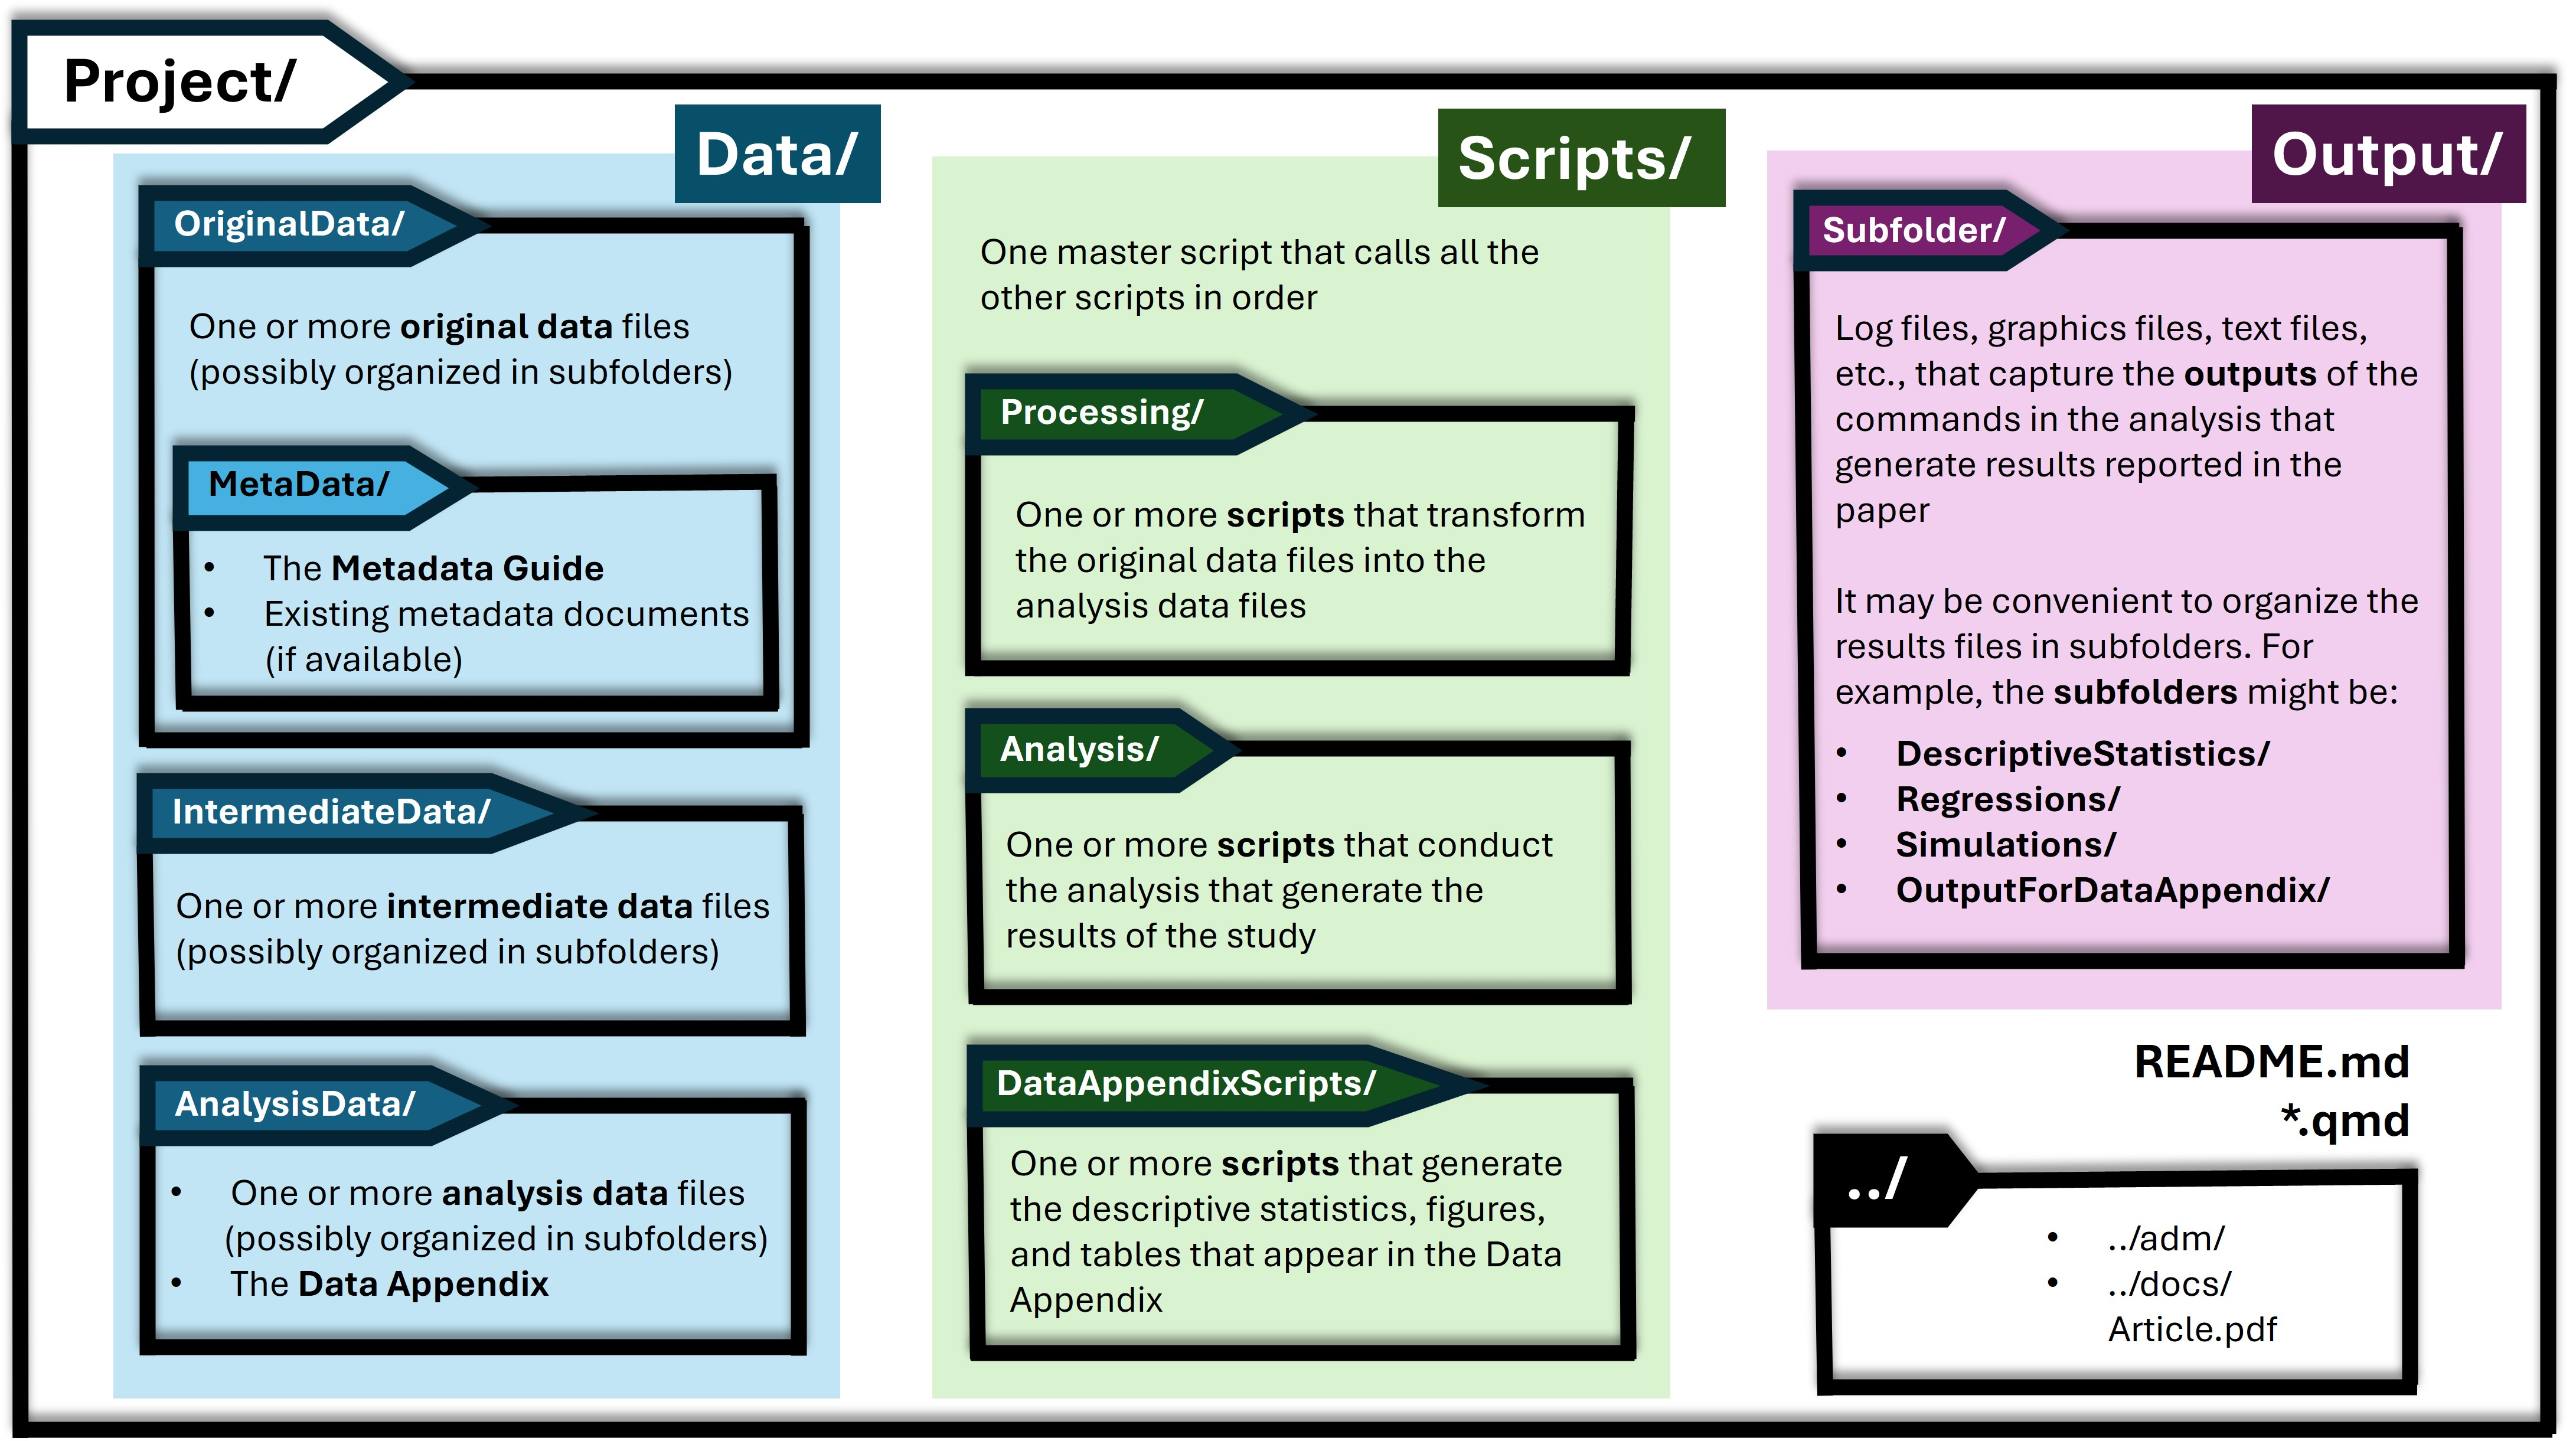
\includegraphics[keepaspectratio]{Output/tier-folders.jpg}}}

\caption{\label{fig-tier-folders}TIER Protocol 4.0: Quarto Reproducible
Dynamic Template. Illustration available at:
https://doi.org/10.5281/zenodo.13119617}

\end{figure}%

For more details about \textbf{TIER Protocol 4.0} visit the page:
\url{https://www.projecttier.org/} and/or read the Domingos \& Batista
(2021) article.

Read the README files for the
\href{https://github.com/phdpablo/article-template/}{project root} and
\href{https://github.com/phdpablo/article-template}{this repository} to
learn more about how this protocol works with this template.

\bookmarksetup{startatroot}

\section{Background}\label{background}

The text below is intended to be an instructive example\ldots{}

Make sure to look into the thought of reproducible research practice
(Dogucu \& Çetinkaya-Rundel, 2022; Gilroy \& Kaplan, 2019; Sullivan et
al., 2019; Vuorre \& Curley, 2018; Wiebels \& Moreau, 2021; Wilson et
al., 2017).

\bookmarksetup{startatroot}

\section{Methods}\label{methods}

The text below is intended to be an instructive example\ldots{}

If you need to learn a little more about Reproducible Research with
R/RStudio there are excellent free e-books:

\begin{itemize}
\item
  \href{https://r4ds.hadley.nz/}{R for Data Science}
\item
  \href{https://raps-with-r.dev/}{Building reproducible analytical
  pipelines with R}
\item
  \href{https://arca-dpss.github.io/manual-open-science/}{The Open
  Science Manual: Make Your Scientific Research Accessible and
  Reproducible}
\end{itemize}

\bookmarksetup{startatroot}

\section{Results}\label{results}

The text below is intended to be an instructive example\ldots{}

Include tables, graphs, figures, and other visual aids from your scripts
in the \texttt{AnalysisScripts} folder as you write up your narrative.
To learn how to complete this integration, look to
\href{https://quarto.org/docs/authoring/notebook-embed.html}{Quarto's
documentation embedding}.

I've included two examples of how to include results from your analytic
scripts into your story below: Figure~\ref{fig-pressure} and
Table~\ref{tbl-diamonds}.

\begin{figure}

\pandocbounded{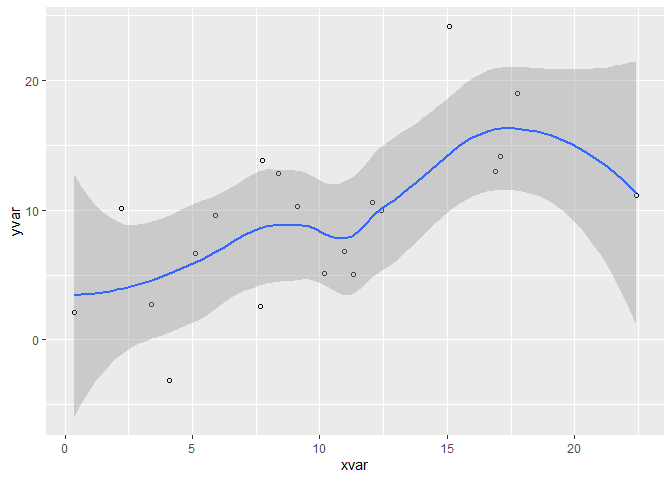
\includegraphics[keepaspectratio]{04-results_files/figure-latex/-Scripts-AnalysisScripts-data_visualization-fig-pressure-output-1.png}}

\caption{\label{fig-pressure}Pressure}

\end{figure}%

\begin{longtable}[]{@{}
  >{\raggedleft\arraybackslash}p{(\linewidth - 18\tabcolsep) * \real{0.0941}}
  >{\raggedright\arraybackslash}p{(\linewidth - 18\tabcolsep) * \real{0.1412}}
  >{\raggedright\arraybackslash}p{(\linewidth - 18\tabcolsep) * \real{0.0941}}
  >{\raggedright\arraybackslash}p{(\linewidth - 18\tabcolsep) * \real{0.1176}}
  >{\raggedleft\arraybackslash}p{(\linewidth - 18\tabcolsep) * \real{0.0941}}
  >{\raggedleft\arraybackslash}p{(\linewidth - 18\tabcolsep) * \real{0.0941}}
  >{\raggedleft\arraybackslash}p{(\linewidth - 18\tabcolsep) * \real{0.0941}}
  >{\raggedleft\arraybackslash}p{(\linewidth - 18\tabcolsep) * \real{0.0824}}
  >{\raggedleft\arraybackslash}p{(\linewidth - 18\tabcolsep) * \real{0.0824}}
  >{\raggedleft\arraybackslash}p{(\linewidth - 18\tabcolsep) * \real{0.0824}}@{}}

\caption{\label{tbl-diamonds}Diamonds characteristics}

\tabularnewline

\toprule\noalign{}
\begin{minipage}[b]{\linewidth}\raggedleft
carat
\end{minipage} & \begin{minipage}[b]{\linewidth}\raggedright
cut
\end{minipage} & \begin{minipage}[b]{\linewidth}\raggedright
color
\end{minipage} & \begin{minipage}[b]{\linewidth}\raggedright
clarity
\end{minipage} & \begin{minipage}[b]{\linewidth}\raggedleft
depth
\end{minipage} & \begin{minipage}[b]{\linewidth}\raggedleft
table
\end{minipage} & \begin{minipage}[b]{\linewidth}\raggedleft
price
\end{minipage} & \begin{minipage}[b]{\linewidth}\raggedleft
x
\end{minipage} & \begin{minipage}[b]{\linewidth}\raggedleft
y
\end{minipage} & \begin{minipage}[b]{\linewidth}\raggedleft
z
\end{minipage} \\
\midrule\noalign{}
\endhead
\bottomrule\noalign{}
\endlastfoot
0.23 & Ideal & E & SI2 & 61.5 & 55 & 326 & 3.95 & 3.98 & 2.43 \\
0.21 & Premium & E & SI1 & 59.8 & 61 & 326 & 3.89 & 3.84 & 2.31 \\
0.23 & Good & E & VS1 & 56.9 & 65 & 327 & 4.05 & 4.07 & 2.31 \\
0.29 & Premium & I & VS2 & 62.4 & 58 & 334 & 4.20 & 4.23 & 2.63 \\
0.31 & Good & J & SI2 & 63.3 & 58 & 335 & 4.34 & 4.35 & 2.75 \\
0.24 & Very Good & J & VVS2 & 62.8 & 57 & 336 & 3.94 & 3.96 & 2.48 \\

\end{longtable}

To learn how it was done, follow the code! Please take note that I was
only referring to the output that was suggested in the
\texttt{data\_visualization.qmd} script located in the
\texttt{Scripts/AnalysisScripts} folder. You can refer to the script for
more information.

\bookmarksetup{startatroot}

\section{Conclusion}\label{conclusion}

The text below is intended to be an instructive example\ldots{}

Although your story must be auditable and replicable by your scripts,
keep in mind that not everything in your scripts needs to be in your
narrative. For example, you may want to include a summary of your
results in your narrative, but you don't need to include all the code
that generated those results. You can include the code in a separate
script file that you reference in your table summary. In this approach,
you can provide the context you need to audit your results within your
repository, all the while keeping your narrative focused on the story
you are trying to tell.

\bookmarksetup{startatroot}

\section*{References}\label{references}
\addcontentsline{toc}{section}{References}

\markboth{References}{References}

\phantomsection\label{refs}
\begin{CSLReferences}{1}{0}
\bibitem[\citeproctext]{ref-dogucu2022}
Dogucu, M., \& Çetinkaya-Rundel, M. (2022). Tools and Recommendations
for Reproducible Teaching. \emph{Journal of Statistics and Data Science
Education}, \emph{30}(3), 251--260.
\url{https://doi.org/10.1080/26939169.2022.2138645}

\bibitem[\citeproctext]{ref-domingos2021}
Domingos, A., \& Batista, I. R. (2021). A map for transparency and
replicability in empirical social science: the TIER Protocol.
\emph{Revista Política Hoje}, 40--86.
\url{https://doi.org/10.51359/1808-8708.2021.245776}

\bibitem[\citeproctext]{ref-gilroy2019}
Gilroy, S. P., \& Kaplan, B. A. (2019). Furthering Open Science in
Behavior Analysis: An Introduction and Tutorial for Using GitHub in
Research. \emph{Perspectives on Behavior Science}, \emph{42}(3),
565--581. \url{https://doi.org/10.1007/s40614-019-00202-5}

\bibitem[\citeproctext]{ref-kathawalla2021}
Kathawalla, U.-K., Silverstein, P., \& Syed, M. (2021). Easing Into Open
Science: A Guide for Graduate Students and Their Advisors.
\emph{Collabra: Psychology}, \emph{7}(1), 18684.
\url{https://doi.org/10.1525/collabra.18684}

\bibitem[\citeproctext]{ref-klein2018}
Klein, O., Hardwicke, T. E., Aust, F., Breuer, J., Danielsson, H., Mohr,
A. H., IJzerman, H., Nilsonne, G., Vanpaemel, W., \& Frank, M. C.
(2018). A Practical Guide for Transparency in Psychological Science.
\emph{Collabra: Psychology}, \emph{4}(1), 20.
\url{https://doi.org/10.1525/collabra.158}

\bibitem[\citeproctext]{ref-sullivan2019}
Sullivan, I., DeHaven, A., \& Mellor, D. (2019). Open and Reproducible
Research on Open Science Framework. \emph{Current Protocols Essential
Laboratory Techniques}, \emph{18}(1), e32.
\url{https://doi.org/10.1002/cpet.32}

\bibitem[\citeproctext]{ref-vuorre2018}
Vuorre, M., \& Curley, J. P. (2018). Curating Research Assets: A
Tutorial on the Git Version Control System. \emph{Advances in Methods
and Practices in Psychological Science}, \emph{1}(2), 219--236.
\url{https://doi.org/10.1177/2515245918754826}

\bibitem[\citeproctext]{ref-wiebels2021}
Wiebels, K., \& Moreau, D. (2021). Leveraging Containers for
Reproducible Psychological Research. \emph{Advances in Methods and
Practices in Psychological Science}, \emph{4}(2), 251524592110178.
\url{https://doi.org/10.1177/25152459211017853}

\bibitem[\citeproctext]{ref-wilson2017}
Wilson, G., Bryan, J., Cranston, K., Kitzes, J., Nederbragt, L., \&
Teal, T. K. (2017). Good enough practices in scientific computing.
\emph{PLOS Computational Biology}, \emph{13}(6), e1005510.
\url{https://doi.org/10.1371/journal.pcbi.1005510}

\end{CSLReferences}




\end{document}
